
%================================
\subsection{Resultados de los algoritmos secuenciales}
\label{sec:Resultados de los algoritmos secuenciales}

En esta sección se presentan los resultados de las cuatro implementaciones secuenciales evaluadas. La versión \textit{base} corresponde a la implementación directa del algoritmo con arreglos de tipo \texttt{int} y sin optimizaciones adicionales; la versión \textit{compiler opt} incorpora optimizaciones de compilación orientadas a mejorar la generación de código; la versión \textit{memory opt} utiliza una representación de memoria más compacta para reducir el consumo y mejorar la localidad de datos; y la versión \textit{compiler + memory opt} combina ambas estrategias con el objetivo de aprovechar simultáneamente mejoras en el cómputo y en el acceso a memoria. A partir de estas variantes se comparan los tiempos de ejecución y se identifica la mejor base secuencial para contrastarla posteriormente con las versiones paralelas.

\begin{table}[H]
   \centering
   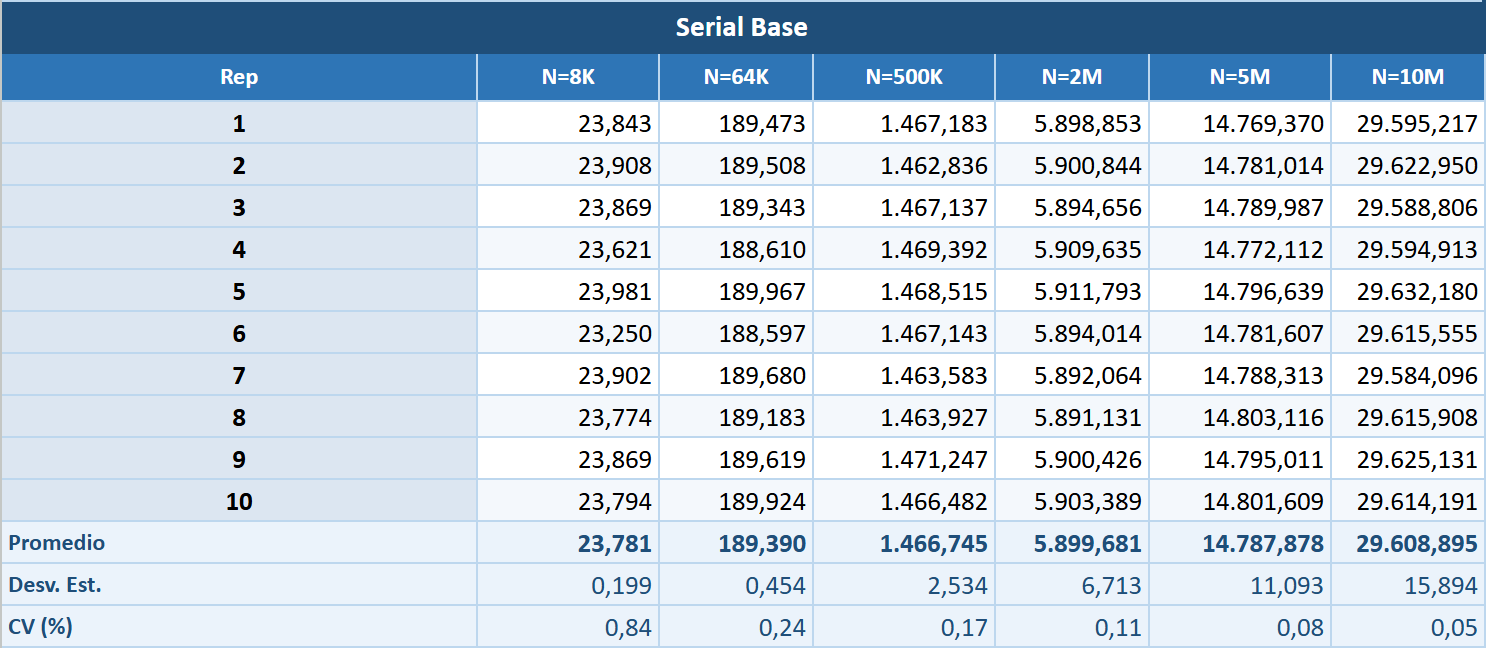
\includegraphics[width=1\textwidth]{images/results/tables/time_seq.png}
   \caption{Tiempos de ejecución del algoritmo secuencial base}
\end{table}

\begin{table}[H]
   \centering
   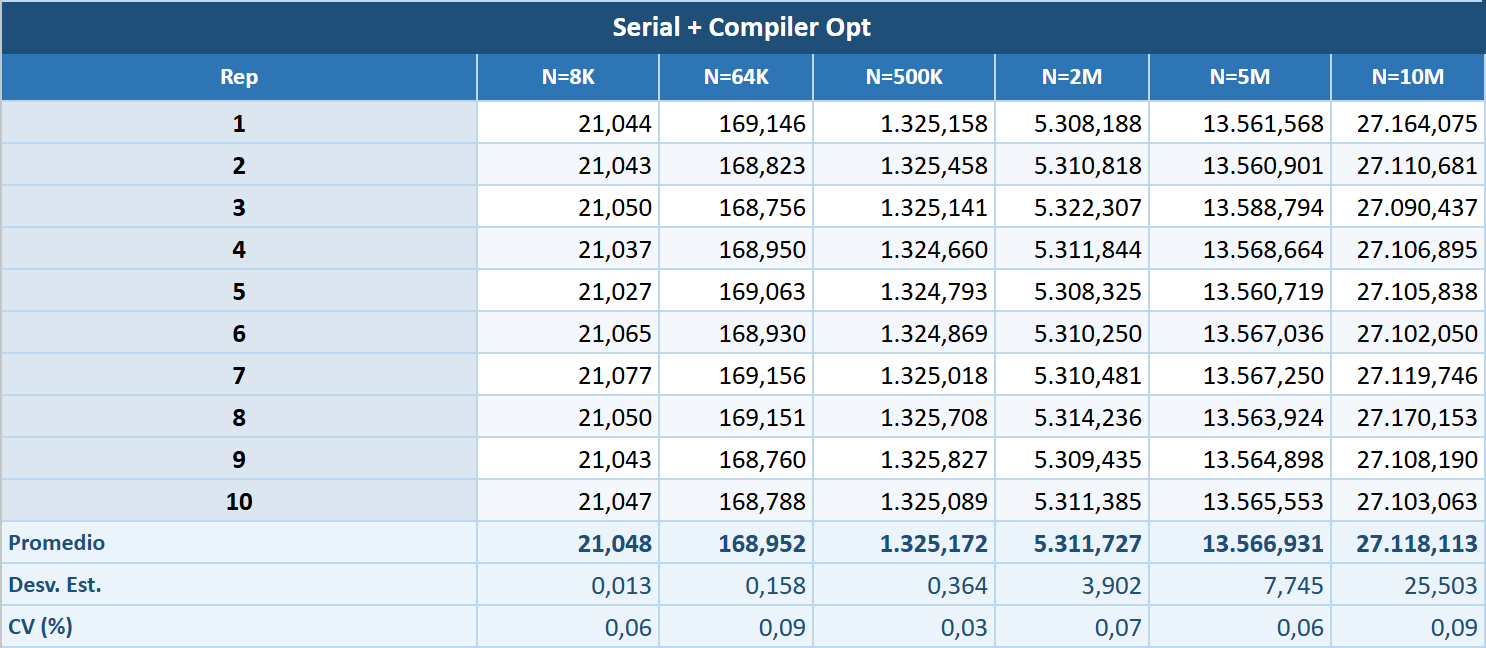
\includegraphics[width=1\textwidth]{images/results/tables/time_seq_opt.png}
   \caption{Tiempos de ejecución del algoritmo secuencial optimizado por compilador}
\end{table}

\begin{table}[H]
   \centering
   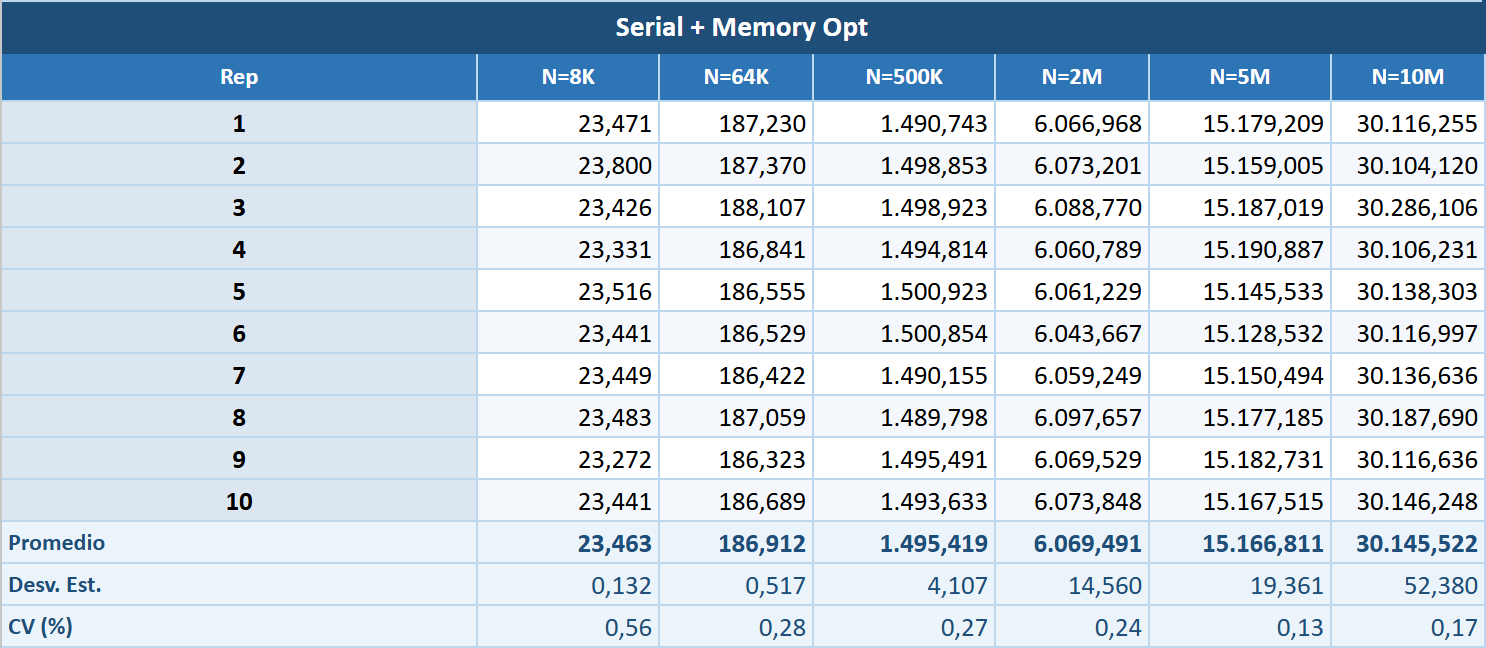
\includegraphics[width=1\textwidth]{images/results/tables/time_seq_mem.png}
   \caption{Tiempos de ejecución del algoritmo secuencial con optimización de memoria}
\end{table}

\begin{table}[H]
   \centering
   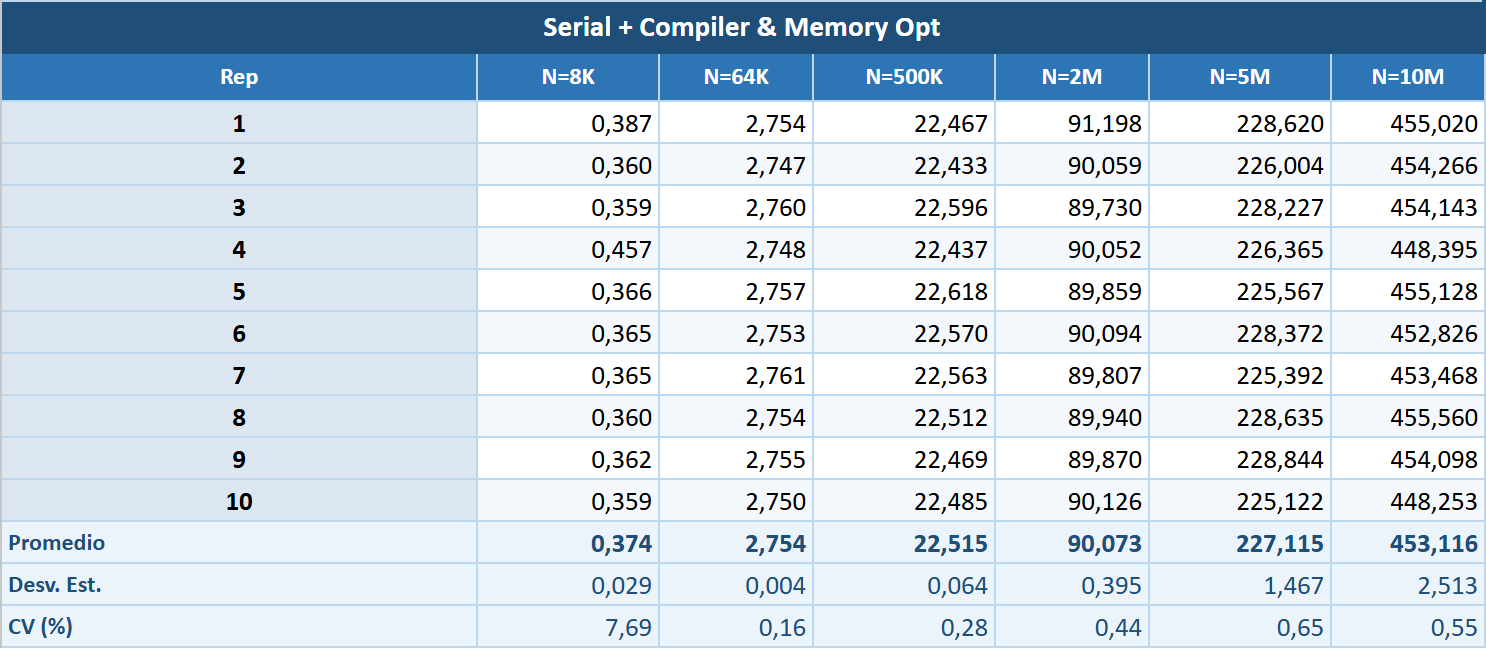
\includegraphics[width=1\textwidth]{images/results/tables/time_seq_opt_mem.png}
   \caption{Tiempos de ejecución del algoritmo secuencial con optimización de memoria y compilador}
\end{table}

\begin{table}[H]
   \centering
   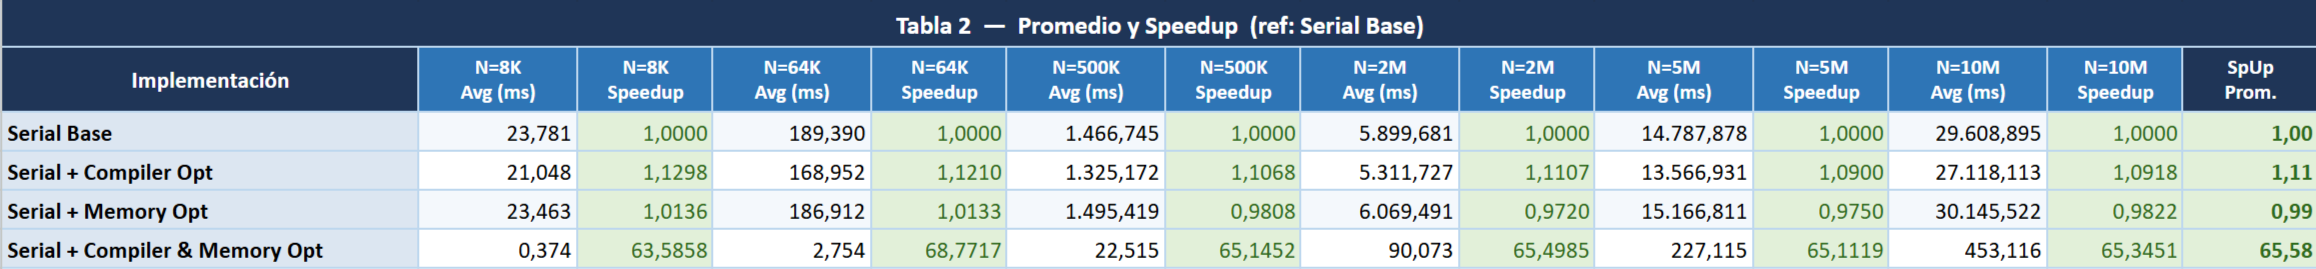
\includegraphics[width=1\textwidth]{images/results/tables/speedup_seq.png}
   \caption{Speedup del algoritmo secuencial base}
\end{table}

\begin{figure}[H]
   \centering
   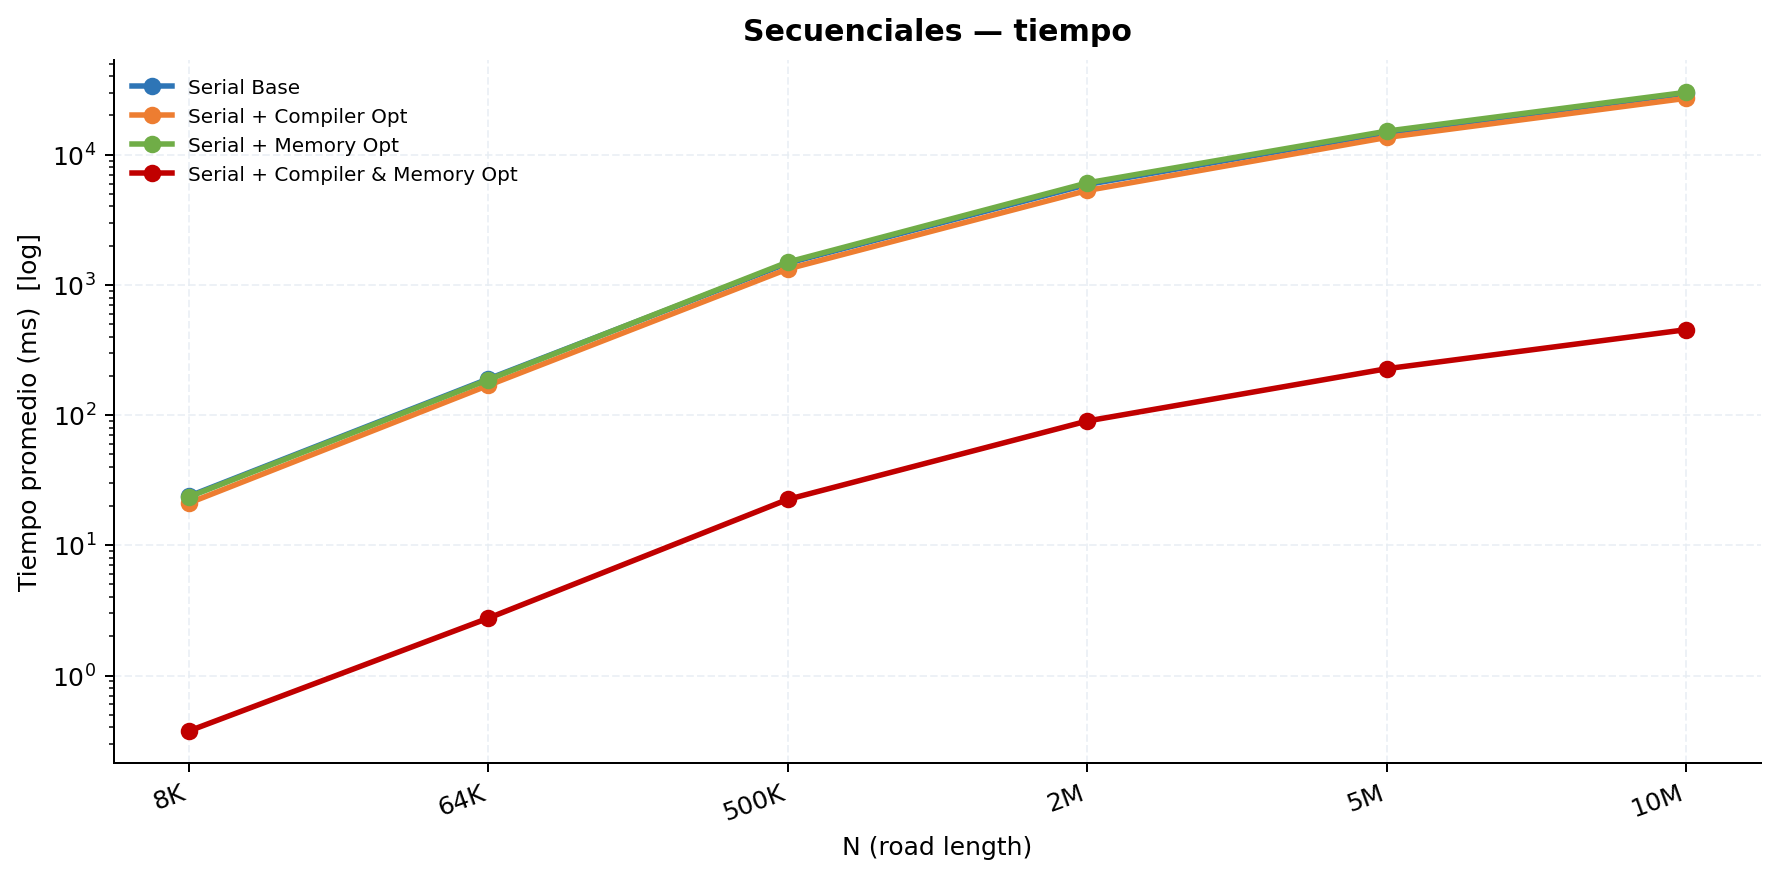
\includegraphics[width=1\textwidth]{images/results/charts/fig_seq_time.png}
   \caption{Tiempos de ejecución de los algoritmos secuenciales}
\end{figure}

\begin{figure}[H]
   \centering
   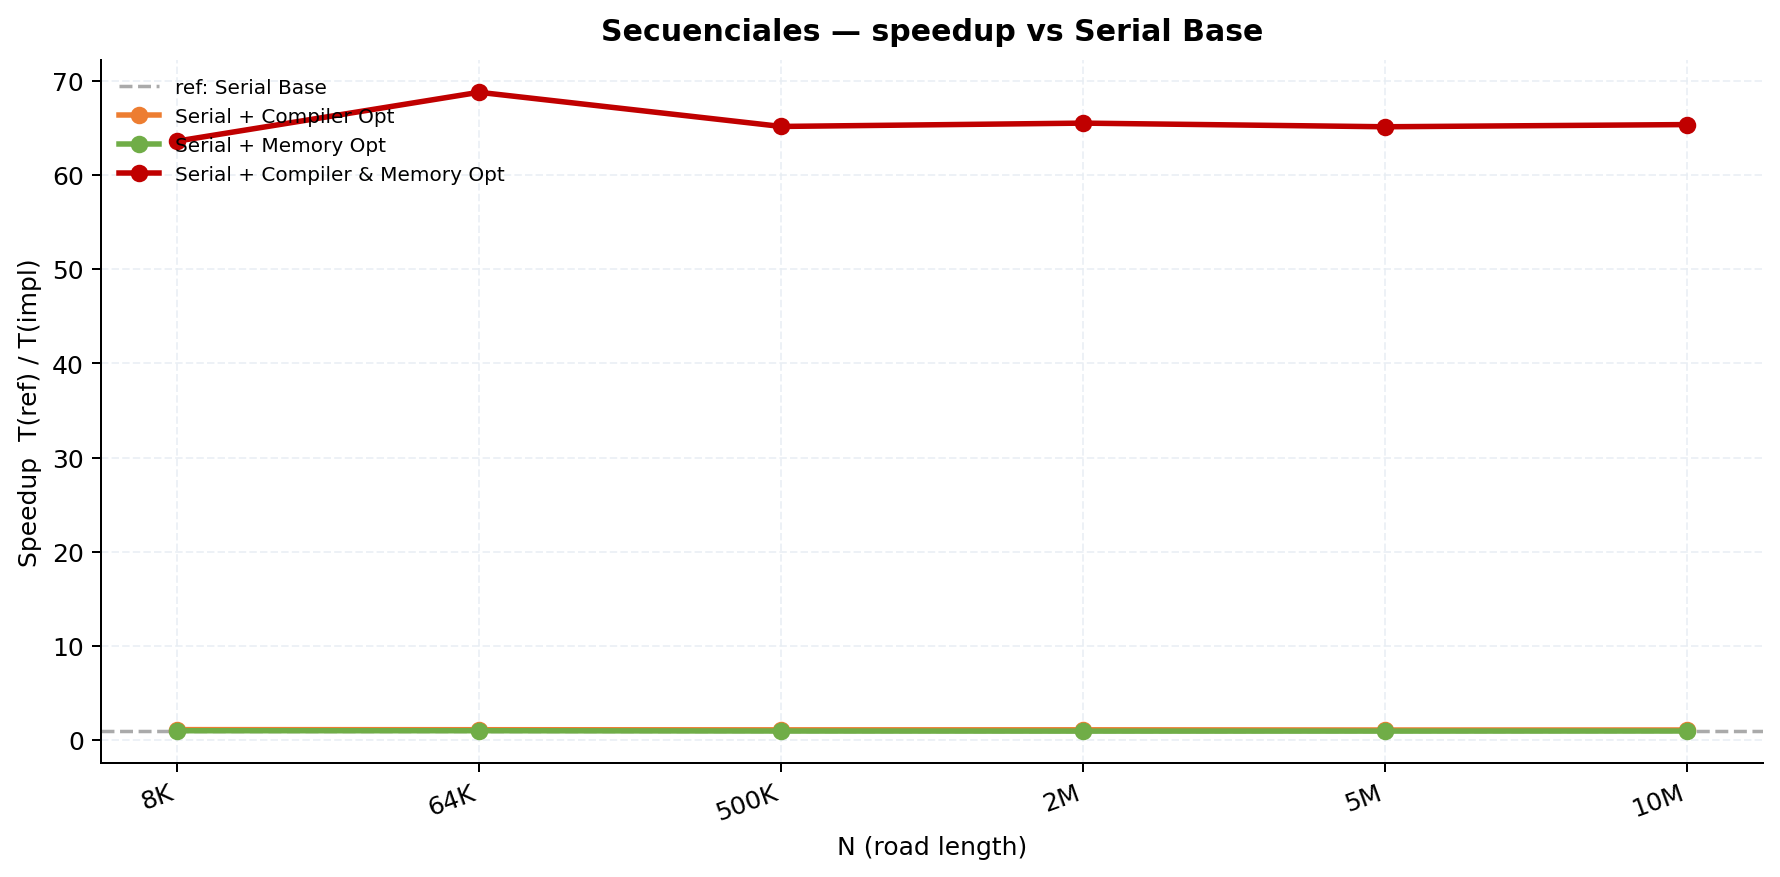
\includegraphics[width=1\textwidth]{images/results/charts/fig_seq_speedup.png}
   \caption{Speedup de los algoritmos secuenciales}
\end{figure}

Como se puede observar la mejor versión secuencial es la que combina optimización de memoria y optimización por compilador, alcanzando un speedup de aproximadamente 65x en comparación con la versión base, lo cual representa una mejora enorme. Esto se debe a que la optimización de memoria reduce significativamente el tiempo de acceso a datos, mientras que las optimizaciones del compilador mejoran la eficiencia del código generado. En contraste, la versión con solo optimización por compilador o solo optimización de memoria muestra mejoras menores, lo que indica que ambas estrategias son complementarias y su combinación es clave para maximizar el rendimiento en este caso. Teniendo esto en cuenta, se seleccionará la versión \textit{compiler + memory opt} como la base secuencial para compararla posteriormente con las implementaciones paralelas y evaluar el impacto de la paralelización sobre el rendimiento.